\chapter{Evaluation}\label{ch:evaluation}
This chapter introduces the methods used for evaluating the system developed in regard to the problem statement. It also describes the procedure of the evaluation. Furthermore it contains the analysis of the results which were obtained from the evaluation.

\section{Objective and Method} 
Set in relation to the problem formulation, the purpose of this evaluation is to learn what effect will the use of AR during a guided tour have on the user experience in comparison to a regular guided tour without the usage of AR. This is done in order to test whether incorporating AR will be beneficial during guided tours or not. 

To test this, two similar versions of a guided tour have been arranged in cooperation with a tour guide from Aalborg Guideforening connected to the project through VisitAalborg - one with AR and one without AR. For the test to not suffer from fatigue by a repetitive experience within the participants testing the two tour versions, the research method between-subjects (often used within the scientific discipline of psychology when comparing two conditions \cite{Charness2012}) was used. This method is used together with the quantitative methodology survey research - used as the primary source for data collection.

The data collected from the questionnaire by rating scales is considered ordinal measurements. To analyse ordinal responses, a nonparametric test is recommended. Moreover, the design of the experiment is unpaired, meaning each participant only tested one of the two tour versions. Because of this, a nonparametric test like the Mann-Whitney U test should be used for the analysis, which will be described more in-depth further into this chapter. For the calculations of the data the significance level has been set to 0.05. The questionnaire can be found in Appendix \ref{app:questionnaire}.

In addition, the qualitative data collection method \textit{semi-structured interview} was utilised to make an in-person interview with the guide after the tour has ended, since interviews are good for tapping into expert knowledge, practices, and opinions \cite{RAND}. The intention of this was to retrieve the guide’s opinions about the usage of AR during the guided tour and the impact it may have had on the tour experience. This provided another source of data with which a triangulation of the results given in the questionnaire answered by the participants can be performed. Furthermore, this data can be used to enrich the quality and the depth of the collected data in order to qualify whether AR and guided tours in practice are compatible or not. The reasoning behind choosing the form \textit{semi-structured} is that it provides detailed information through a somewhat conversational style. It still lets the interviewer have a certain control over the interview through some prepared questions and topics from which to structure and guide the direction \cite{RAND}.

Both the tours and the interview have been recorded on video for documentation and further analysis. For the the video recording method \textit{shadowing} is used as this excels as a method for observing people while they move and perform their routine \cite{Ylirisku2007}. During the evaluation, both the participants and guide has been shadowed by a camera. The first has been done to later enable an analysis of whether or not the results from the questionnaires, which were given by the participants, are consistent with what was observed by the camera. Meanwhile, the reason for having the guide followed was to see if the content presented by her could be considered similar to the two tours in order to eliminate this as a factor to influence the result. Another reason for following the guide with a camera was to see if her routine changes when the application is added, as to see if she is impacted by it.

\subsection{Hypotheses}\label{sec:hypotheses}
The following hypotheses are formed based on the latter three research questions presented in Chapter \ref{ch:problemstatement}. The following hypothesis is formed based on research question 2: \textit{In what way does the addition of an AR application affect tour goers’ curiosity to learn more, if at all?}

\paragraph{H1\textsubscript{0}:} After experiencing a tour with the AR application, participants report the same level of curiosity as that of the participants who experienced the tour without the AR application.

\paragraph{H1\textsubscript{a}:}  After experiencing a tour with the AR application, participants report a different level of curiosity than that of the participants who experienced the tour without the AR application.\pagebreak

If the null hypothesis H1\textsubscript{0} is rejected and the alternative hypotheses H1\textsubscript{a} is found to be true, an additional hypothesis may be tested, examining the nature of the difference between the two groups of participants:

\paragraph{H1\textsubscript{b}:} After experiencing a tour with the AR application, participants report a higher level of curiosity than that of the participants who experienced the tour without the AR application.\\
\\
The following hypothesis is formed based on research question 3: \textit{In what way does the addition of an AR application affect whether tour goers find the tour entertaining, if at all?}

\paragraph{H2\textsubscript{0}:} After experiencing a tour with the AR application, participants report the same level of entertainment as that reported by the participants who experienced the tour without the AR application.

\paragraph{H2\textsubscript{a}:} After experiencing a tour with the AR application, participants report a different level of entertainment as that reported by the participants who experienced the tour without the AR application.\\
\\
If the null hypothesis H2\textsubscript{0} is rejected and the alternative hypotheses H2\textsubscript{a} is found to be true, an additional hypothesis may be tested, examining the nature of the difference between the two groups of participants:

\paragraph{H2\textsubscript{b}:} After experiencing a tour with the AR application, participants report a higher level of entertainment compared to that reported by the participants who experienced the tour without the AR application.\\
\\
Lastly, the following hypotheses are formed based on research question 4: \textit{In what way does the addition of an AR application affect whether tour goers are distracted during the tour?}

\paragraph{H3\textsubscript{0}:} After experiencing a tour with the AR application, participants report the same level of distraction as that of the participants who experienced the tour without the AR application.

\paragraph{H3\textsubscript{a}:}After experiencing a tour with the AR application, participants report a different level of distraction than that of the participants who experienced the tour without the AR application.\pagebreak

If the null hypothesis H3\textsubscript{0} is rejected and the alternative hypotheses H3\textsubscript{a} is found to be true, an additional hypothesis may be tested, examining the nature of the difference between the two groups of participants:

\paragraph{H3\textsubscript{b}:} After experiencing a tour with the AR application, participants report a higher level of distraction than that of the participants who experienced the tour without the AR application.\\
\\
To better understand the system of hypotheses, a flowchart can be seen in Figure \ref{fig:hypo_flowchart}. If H\textsubscript{a} is rejected, H\textsubscript{0} is accepted. However, if H\textsubscript{a} is accepted, H\textsubscript{b} can be investigated, examining the nature of the difference found.

\begin{figure}[h!]
  \centering
  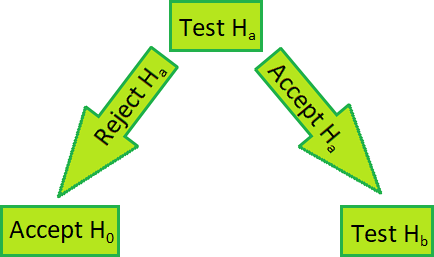
\includegraphics[scale=0.4]{figures/hypo_flowchart.png}
  \caption{A flowchart showing how to proceed depending on the results for H\textsubscript{a}}\label{fig:hypo_flowchart}
\end{figure}

These hypotheses will be examined in the analysis of the results further into this chapter. The statistical analyses assume a confidence level of 95 for all of these hypotheses.

\section{Participants}
The participants were acquired through the use of a facebook event and personal enquiry. They were mainly among friends and acquaintances of the group members.  
The participants in this test were all people aged 20-31, who volunteered to participate in the experiment. A visualisation of the age distribution can be seen in Figure \ref{fig:age}. The control group consisted of 7 men and 4 women, and the test group consisted of 9 men and 4 women. All participants were informed that they would be filmed, and that they had the right to withhold any information or answers gathered during the test, and that they could withdraw their consent to participate at any time.

\begin{figure}[h!]
  \centering
  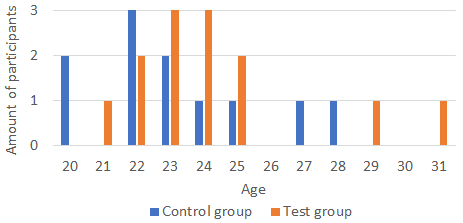
\includegraphics[scale=0.7]{figures/agedistribution.png}
  \caption{The age distribution of the participants in the two groups}\label{fig:age}
\end{figure}

Aside from the volunteers, a tour guide from Aalborg Guideforening participated in the test, in order to properly simulate a guided tour.

\section{Setting and procedure}
The test consisted of a guided tour of app. 30 minutes, with two groups of participants. It took place in Aalborg city centre during the morning. The guide was Inge Vestergaard from Aalborg Guideforening. The guided tour started at Gammeltorv, then continued onto the area where Rakkerens Hule was located. There, one group experienced the AR application. This group is referred to as the \textit{test group}, and the other is the \textit{control group}. The tour finished off at the old monastery Helligåndsklosteret before returning to Gammeltorv. The route can be seen in Figure \ref{fig:map}.

\begin{figure}[h!]
   \centering
   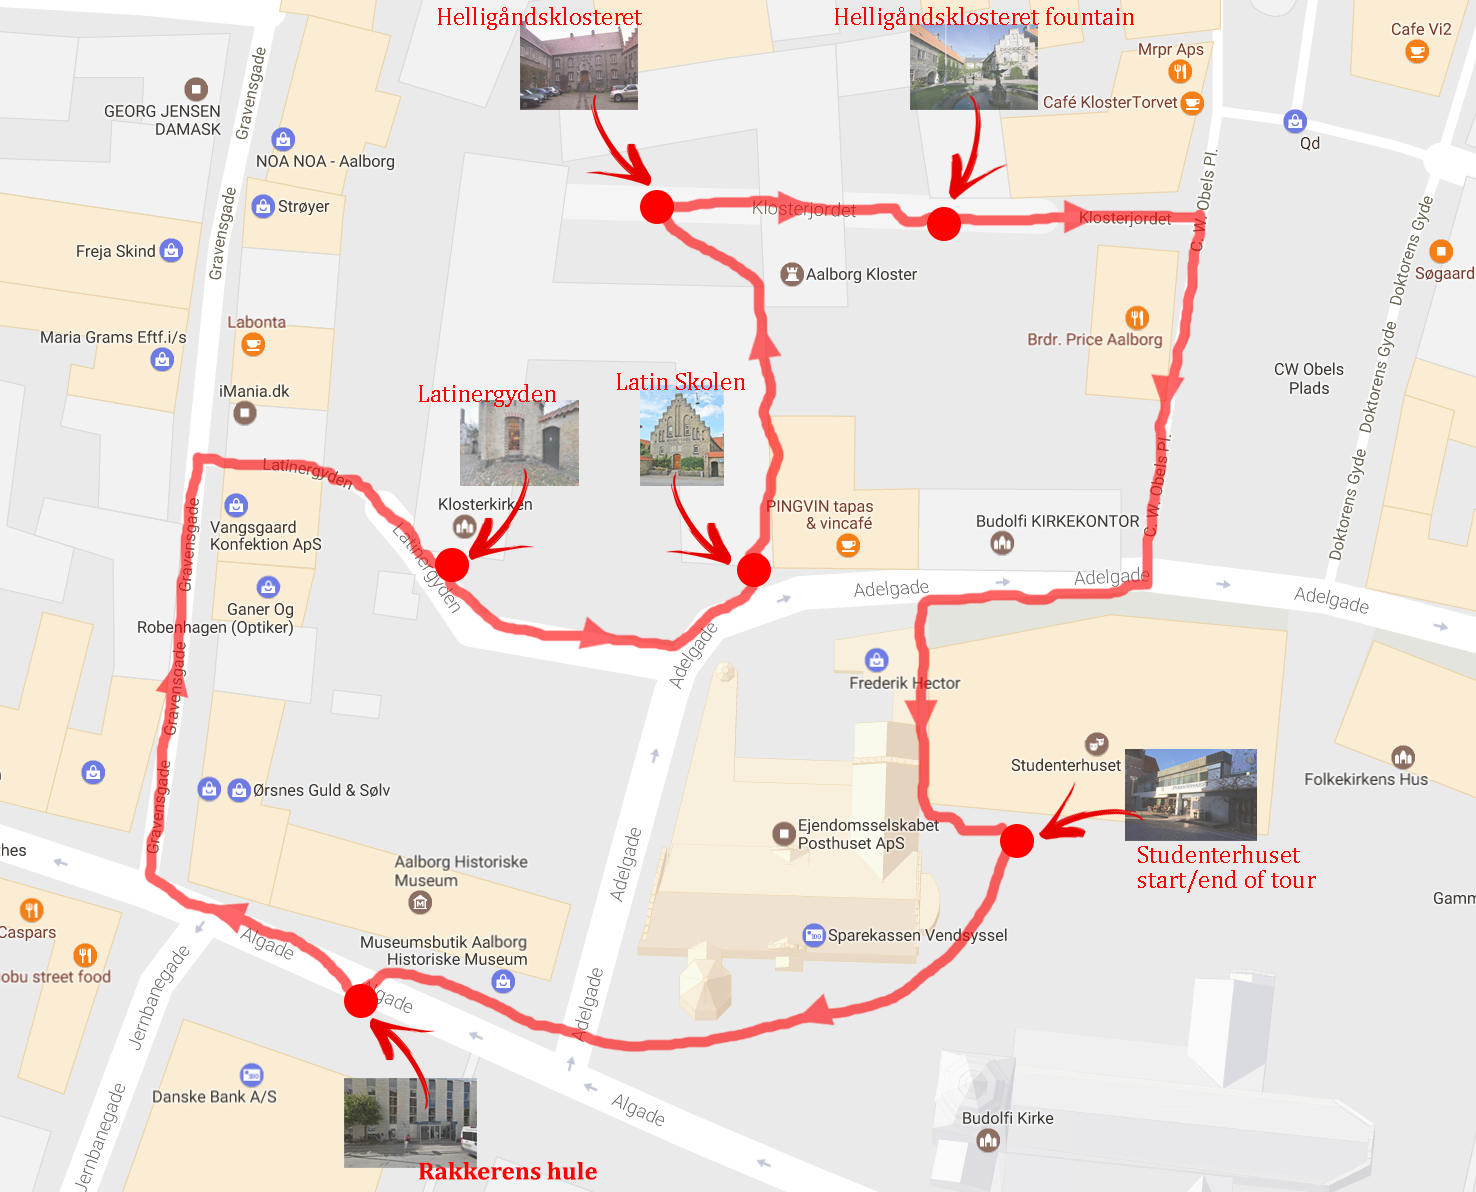
\includegraphics[width=0.8\textwidth]{figures/Tour_map.png}
   \caption{The tour route}\label{fig:map}
\end{figure}

For the test, a timeline was created since the test was only being conducted once and it required coordination with the guide, the project group and the participants. The participants were split into two groups beforehand, so that the second group would not have to wait for the first group to finish. The timeline consisted of the following events:

\begin{figure}[h!]
   \centering
   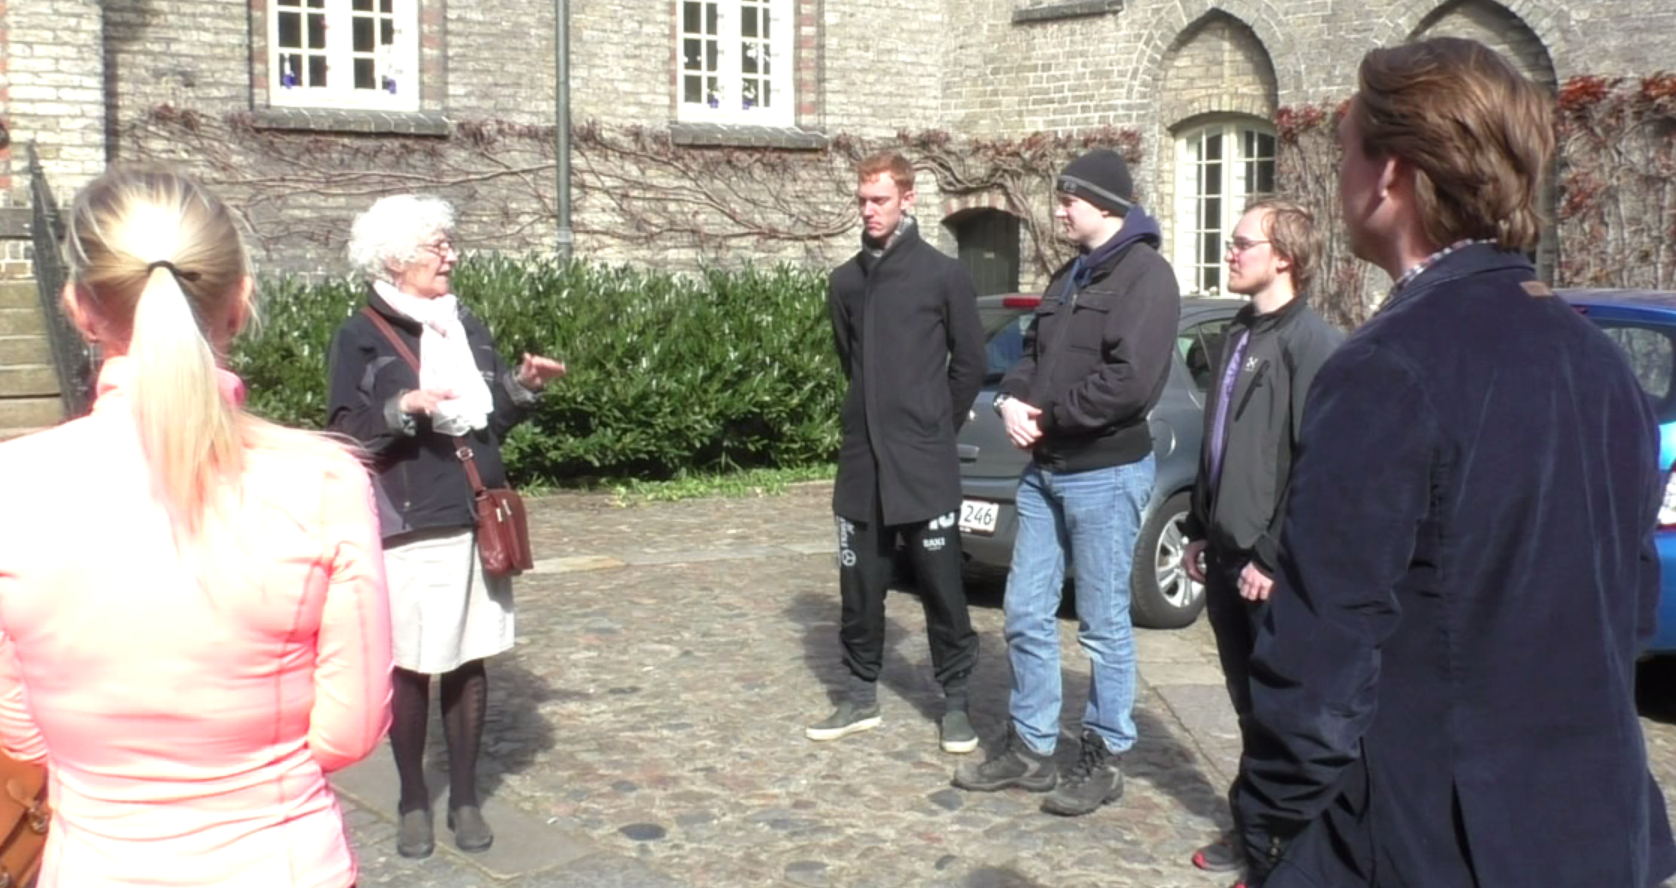
\includegraphics[width=\textwidth]{figures/participants_listen.png}
   \caption{Test participants listening to the tour guide}\label{fig:participants_listen}
\end{figure}

\begin{tabular}{l p{12cm}}
09:00 & - The project group meets up at Gammeltorv to prepare \\
09:45 & - The control group meet up at Gammeltorv \\
 & - Consent forms are presented and the procedure is explained \\
10:00 &   - The control group starts the guided tour \\
10:10 & - The test group meets up at Gammeltorv \\
 & - Consent forms are presented and the procedure is explained including the AR application \\
10:30 & - The control group finishes the guided tour and are handed the questionnaires \\
 & - The test group starts the guided tour
\\ 
11:00 & - The test group finishes the guided tour and are handed the questionnaires \\
 & - The guide is interviewed \\
11:10 & - When the test group is finished the test ends \\
\end{tabular}\pagebreak

\begin{figure}[h!]
   \centering
   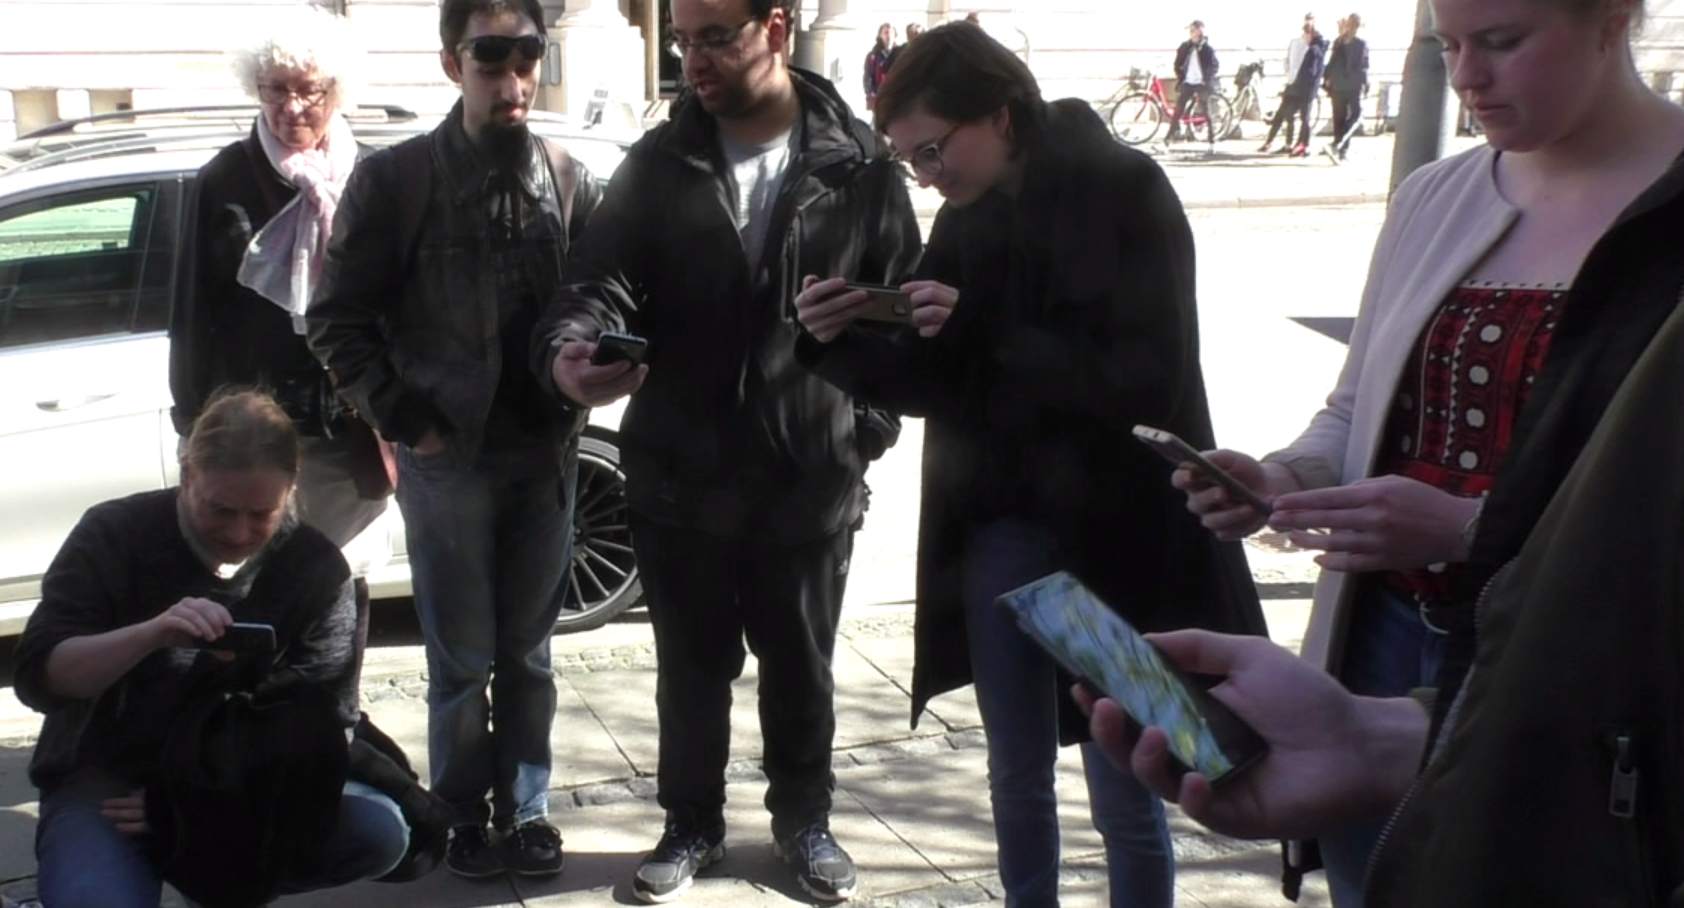
\includegraphics[width=\textwidth]{figures/participants_app.png}
   \caption{Test participants experiencing the AR application}\label{fig:participants_app}
\end{figure}

During the test, two group members followed the tour with video cameras and the necessary marker for the AR application. The other two group members stayed at Gammeltorv to prepare the second group and to be ready to hand out the questionnaires to the first group. Therefore, the required items for the test were as follows:

\begin{itemize}
\item Two video cameras
\item A marker for the AR application
\item Questionnaires
\item Consent forms
\item The participants’ Android phones
\item Clipboards for the questionnaires
\end{itemize}

\section{Statistical analysis of results} 
\subsection{Questionnaire results}
In order to properly analyse the results gathered from the rating scale questions, each possible answer is given a value from -3 to 3, such that -3 corresponds to \textit{strongly disagree}, 0 corresponds to \textit{neither agree nor disagree}, and 3 corresponds to \textit{strongly agree}. This way, a higher level of agreement to a given statement from the questionnaire means a higher value, and the data can be interpreted as ordinal data. The results from the rating scale questions can be seen in Appendix \ref{app:questionnaire_results}.
 
Similarly, each SAM image is given a value from 1 to 5. Since only two of the SAM questions are included in the questionnaire, this means that in the first question, 1 corresponds to \textit{most pleased}, and 5 corresponds to \textit{least pleased}. In the second question, 1 corresponds to \textit{most aroused}, and 5 corresponds to \textit{least aroused}. The results from the SAM questions can be seen in Appendix \ref{app:questionnaire_results}.

\begin{figure}[h!]
   \centering
   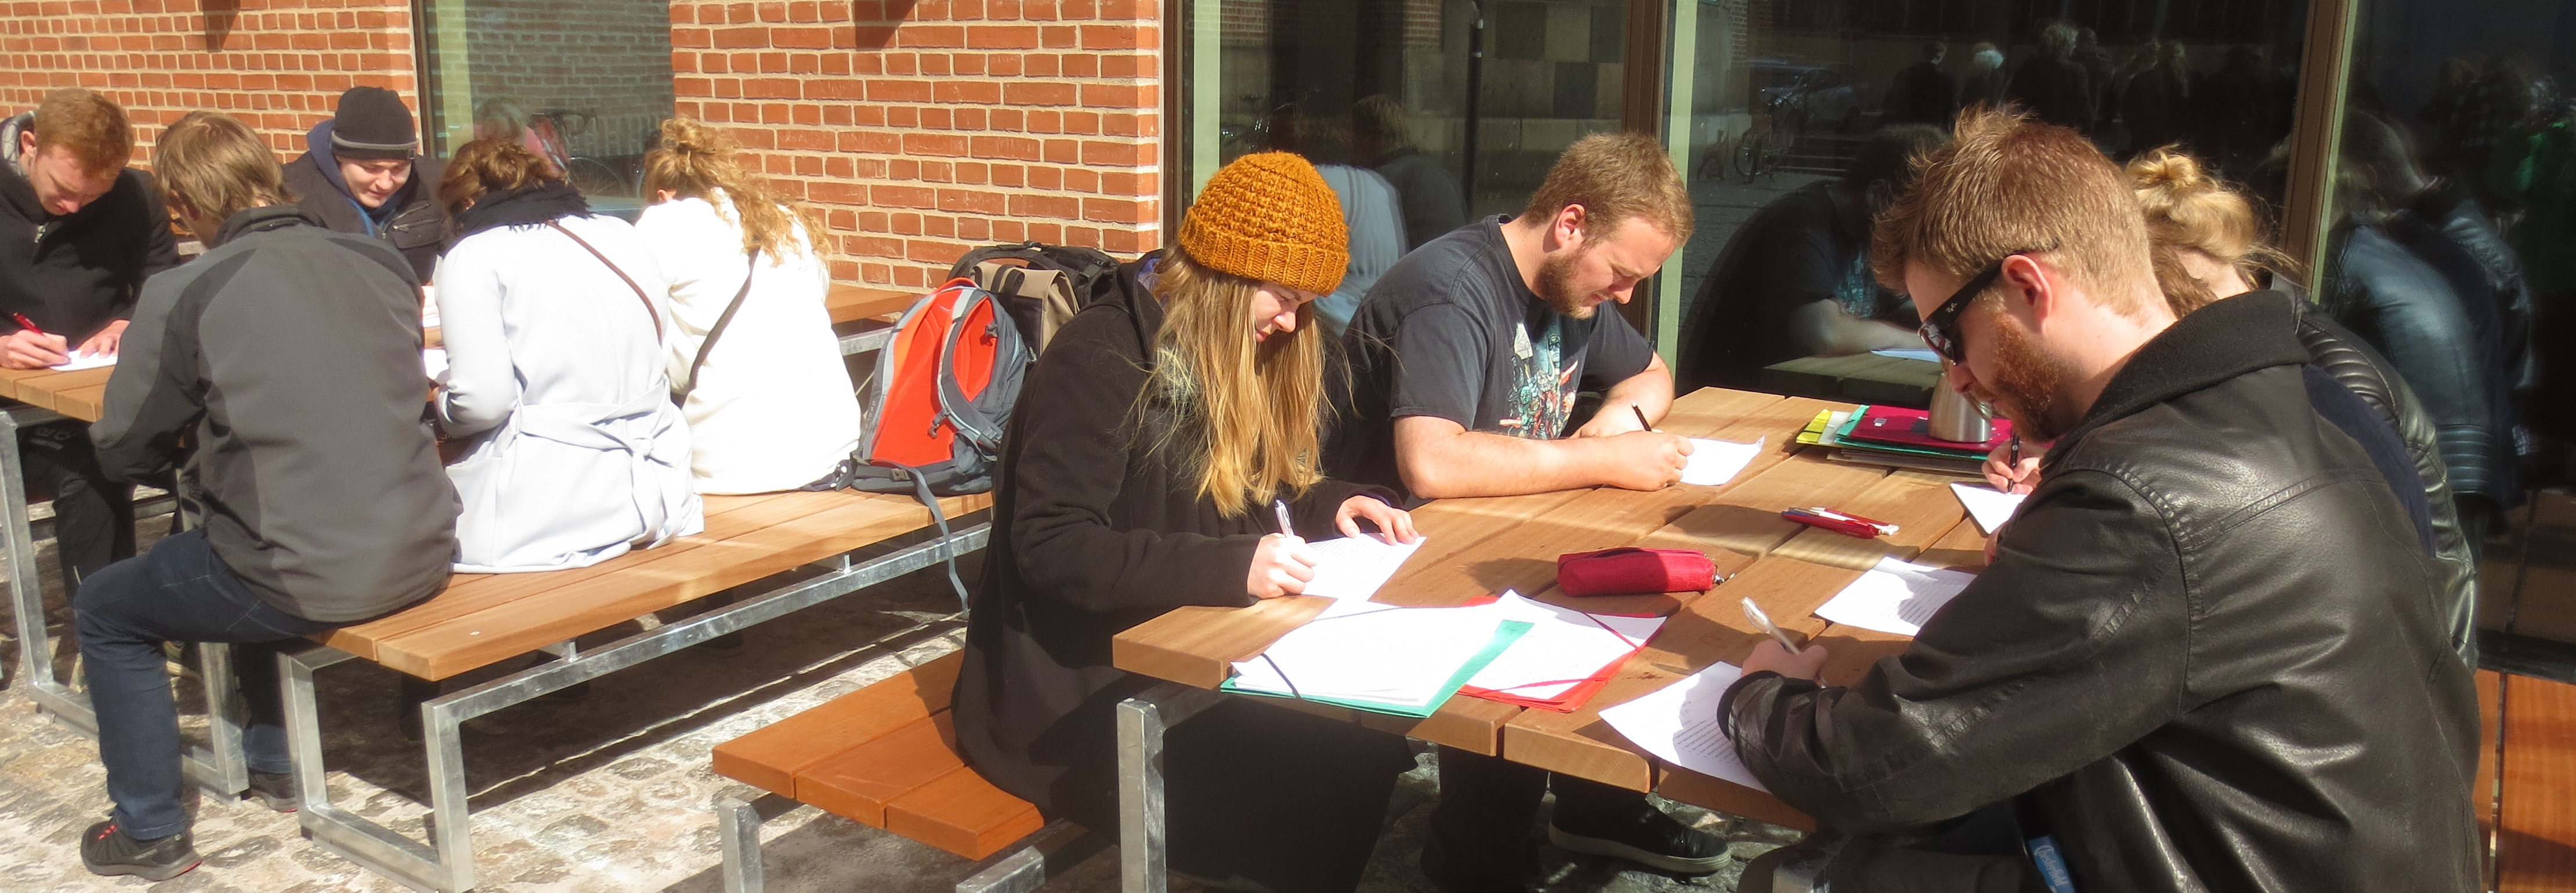
\includegraphics[width=\textwidth]{figures/participants_questionnaire.jpg}
   \caption{Test participants filling out questionnaires}\label{fig:participants_questionnaire}
\end{figure}
 
Lastly, test participants were able to add any comments if they pleased. In this section of the questionnaire, several participants from both the control and the test group stated that noise from traffic at the test site was a distracting factor to them, and that sometimes this made it hard to hear what the guide was saying. However, members of both groups found that the tour proceeded in a nice tempo, and that it was nice to be able to ask questions to an informed person such as the guide. Some participants stated that they were unsure of the meaning of the word ‘aroused’ in the context of this test. A member of the control group expressed that they lacked a visual of the dungeon described by Rakkerens Hule. As for the test group who did see the visual representation, some participants provided feedback regarding the quality of the application. One participant found that the application had difficulty showing the dungeon at certain angles, making it hard to see anything, as the amount of people in the group inhibited their ability to get a good angle. Another participant reported an issue that the model in the application ‘jiggled’ at times. One participant stated that they liked the idea of the application, but would have preferred a version without a marker.
 
The analysis of the results is presented in the following paragraph.

\subsection{Analysis of questionnaire results}\label{sec:questionnaire_analysis}
To compare the questionnaire results of the control and the test group, the Mann-Whitney U test, also known as the Wilcoxon rank-sum test, was utilised. The Mann-Whitney U test was originally conceived by Mann and Whitney in 1947 \cite{Mann1947}, and tests for differences between two groups on a single, ordinal, non-parametric variable. As this is the type of variable which is to be compared between two non-paired samples, this type of test is fitting.

As an example of how this test works, results from the first question will be compared between the control group and the test group. The responses for this particular question can be seen in Table \ref{table:question_1}.

\begin{table}[h!]\centering
\begin{tabular}{| p{1.5cm} | p{0.2cm} | p{0.2cm} | p{0.2cm} | p{0.2cm} | p{0.2cm} | p{0.2cm} | p{0.2cm} | p{0.2cm} | p{0.2cm} | p{0.2cm} | p{0.2cm} | p{0.2cm} | p{0.2cm} |}\hline
\textbf{Control Group} & 2 & 2 & 2 & 3 & 0 & 1 & 1 & 2 & 1 & 0 & 2 &  &  \\ \hline
\textbf{Test Group} & 2 & 0 & 2 & 3 & 3 & 2 & 2 & 0 & 3 & 1 & 1 & 1 &2 \\ \hline
\end{tabular}
\caption{Responses from Question 1 of the questionnaire \label{table:question_1}}
\end{table}

In order to conduct the test, one must find the \textit{U} value, also known as the \textit{ranked sum} value, for each of the two groups. To do this, each response in one sample must be compared to each response in the other sample. The first response of the control group has a value of 2. When comparing this value to the responses of the test group, it is clear that it is higher than some of these values, lower than some, and equal to some. For each value in the test group which is lower than 2, 1 is added to the first response's \textit{rank}, denoted \textit{R\textsubscript{1}}. For each value in the test group equal to 2, 0.5 is added to \textit{R\textsubscript{1}}, and for each value in the test group higher than 2, 0 is added to \textit{R\textsubscript{1}}. This calculation can be seen in Equation \ref{eq:R1}, and results in a rank of \textit{R\textsubscript{1}} = 7.5.

\begin{equation}
\label{eq:R1}
R_1 = 0.5 + 1 + 0.5 + 0 + 0 + 0.5 + 0.5 + 1 + 0 + 1 + 1 + 1 + 0.5 = 7.5
\end{equation}

This calculation is done for every response in the control group. The sum of all ranks in a group, U, is called the ranked sum. The calculation for the ranked sum of the control group, \textit{U\textsubscript{a}}, is seen in Equation \ref{eq:Ua}.

\begin{equation}
\label{eq:Ua}
U_a = 7.5 + 7.5 + 7.5 + 11.5 + 1 + 3.5 + 3.5 + 7.5 + 3.5 + 1 + 7.5 = 61.5
\end{equation}

The same calculations are done for the test group. First, each response's rank is found by comparing the value to each response in the control group. Next, the ranked sum \textit{U\textsubscript{b}} is calculated as seen in Equation \ref{eq:Ub}.

\begin{equation}
\label{eq:Ub}
U_b = 7.5 + 1 + 7.5 + 10.5 + 10.5 + 7.5 + 7.5 + 1 + 10.5 + 3.5 + 3.5 + 3.5 + 7.5 = 81.5
\end{equation}

Only the lowest \textit{U} value is used, which in this case is \textit{U\textsubscript{a}} = 61.5. This value is compared to the \textit{critical ranked sum}, \textit{U\textsubscript{crit}}, which depends on the number of responses in each of the two samples. The appropriate value is looked up in the table seen in Figure \ref{fig:mann_table}. This table applies only to two-tailed Mann-Whitney U tests with an alpha value of 0.05, which is fitting for this test, as the confidence level is 95.

\begin{figure}[h!]
   \centering
   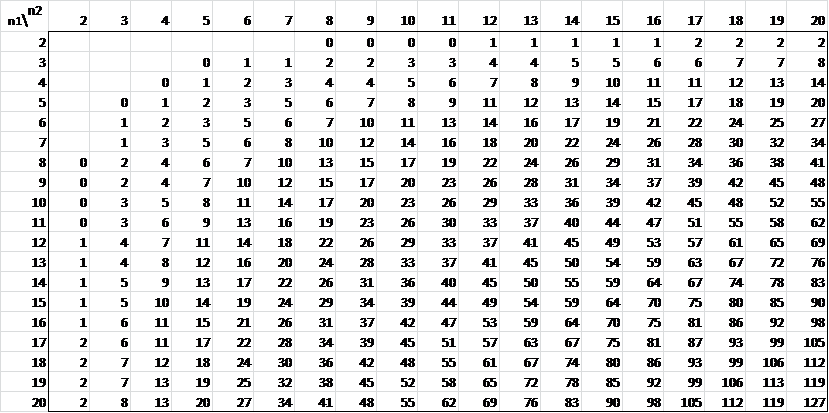
\includegraphics[width=\textwidth]{figures/mann_table.png}
   \caption{Table containing the critical ranked sums depending on number of responses, for a two-tailed test with an alpha value of 0.05 \cite{Utable}}\label{fig:mann_table}
\end{figure}

The sample sizes are 11 and 13 respectively, which means that \textit{U\textsubscript{crit}} = 37. For the Mann-Whitney U test to show a significant difference between two samples, \textit{U} must be lesser than \textit{U\textsubscript{crit}}. Since \textit{U\textsubscript{a}} > \textit{U\textsubscript{crit}}, no significant difference is found between the two samples of responses for Question 1 in the questionnaire.

Doing these calculations by hand are a lengthy process, so in order to simplify, the calculations have instead been done using R, a programming language for statistical computing. The responses for each question are entered as a vector. An example of how this is done can be seen in Listing \ref{lst:entervalues}.

\begin{lstlisting}[language=C, numbers=left, caption={Responses for question 1 are entered for the control group (\texttt{Q1a}) and the test group (\texttt{Q1b}) respectively}, label=lst:entervalues, captionpos=b]
Q1a = c(2,2,2,3,0,1,1,2,1,0,2)
Q1b = c(2,0,2,3,3,2,2,0,3,1,1,1,2)
\end{lstlisting}\pagebreak

Once all data sets are entered, the Mann-Whitney U test can be run by using the \texttt{wilcox.test} function. Listing \ref{lst:wilcox} shows how the \texttt{wilcox.test} function is used to compare the two response samples for question 1.

\begin{lstlisting}[language=C, numbers=left, caption={A two-tailed Mann-Whitney U test using the samples Q1a and Q1b, with a confidence level of 95}, label=lst:wilcox, captionpos=b]
wilcox.test(Q1a, Q1b, alternative = "two.sided", conf.level = 0.95)
\end{lstlisting}

When this test is run, it output a \textit{U} value of \textit{U} = 61.5, which is the same as the one previously calculated by hand. Furthermore, it outputs a p value of p = 0.5627. For the statistical analysis of the questionnaire results, R will be used to analyse tha data gathered from the questionnaires.
 
The first hypothesis is tested: \textit{H1\textsubscript{a}}: After experiencing a tour with the AR application, participants report a different level of curiosity than that of the participants who experienced the tour without the AR application. To test this, results from questions 1-4 of the questionnaire are used (see Appendix \ref{app:questionnaire}). These are compared using the Mann-Whitney U test. Using this test, we investigate whether there is a significant difference between the two results. For the four questions, this test resulted in the following:

\paragraph{Question 1:} p = 0.5627, \textit{U} = 61.5
\paragraph{Question 2:} p = 0.9506, \textit{U} = 70
\paragraph{Question 3:} p = 0.2357, \textit{U} = 51.5
\paragraph{Question 4:} p = 0.9491, \textit{U} = 63.5\\
\\
In all of these cases, p > 0.05 and \textit{U} > 37, and therefore the null hypothesis must be accepted: \textit{H1\textsubscript{0}: After experiencing a tour with the AR application, participants report the same level of curiosity as that of the participants who experienced the tour without the AR application}. Since no significant difference is found, it makes little sense to investigate which sample reported the higher level of curiosity.

Likewise, the second hypothesis is tested: \textit{H2\textsubscript{a}: After experiencing a tour with the AR application, participants report the same level of entertainment as that reported by the participants who experienced the tour without the AR application.} Questions 5 and 11 pertain to the entertainment value of the tour, and questions 6-10 pertain to the quality of the tour. The Mann-Whitney U test is used to test whether there is a significant difference between the two samples when it comes to the following questions.\pagebreak

\paragraph{Question 5:} p = 0.9476, \textit{U} = 73
\paragraph{Question 6:} p = 0.6912, \textit{U} = 78
\paragraph{Question 7:} p = 0.8489, \textit{U} = 75
\paragraph{Question 8:} p = 0.2859, \textit{U} = 53.5
\paragraph{Question 9:} p = 0.2785, \textit{U} = 88
\paragraph{Question 10:} p = 0.8264, \textit{U} = 75.5
\paragraph{Question 11:} p = 0.1702, \textit{U} = 49\\
\\
Once again, for all of these questions, p > 0.05 and \textit{U} > 37, and therefore the null hypotheses must be accepted: \textit{H2\textsubscript{0}: After experiencing a tour with the AR application, participants report a different level of entertainment as that reported by the participants who experienced the tour without the AR application.}

Question 12: “I could see a relation between what I was viewing and what the guide was talking about” does not relate to one of the hypotheses presented in section \ref{sec:hypotheses}, but is nonetheless relevant to the problem statement. Therefore, the Mann-Whitney U test is applied to the responses from this question as well to see if there is a significant difference between the two samples, resulting in p = 0.1448 and \textit{U} = 47.5. Since p > 0.05 and \textit{U} > 37, no significant difference is observed. 

The last hypothesis is \textit{H2\textsubscript{a}: After experiencing a tour with the AR application, participants report a different level of distraction than that of the participants who experienced the tour without the AR application.} This relates to questions 13-16, the responses for which are also compared through a Mann-Whitney U test, resulting in the following:

\paragraph{Question 13:} p = 0.3137, \textit{U} = 54,5
\paragraph{Question 14:} p = 0.4802, \textit{U} = 84
\paragraph{Question 15:} p = 0.7892, \textit{U} = 66.5
\paragraph{Question 16:} p = 0.2648, \textit{U} = 47.5\\
\\
For all of these questions, p > 0.05 and \textit{U} > 37, meaning that no significant difference is observed, and the null hypothesis must be accepted: \textit{H3\textsubscript{0}: After experiencing a tour with the AR application, participants report the same level of distraction as that of the participants who experienced the tour without the AR application.}

The last two questions of the questionnaire are SAM-mannekin based questions, asking participants to mark the image which best represents how pleased and aroused they were, respectively. The Mann-Whitney U test is used on the responses from these two questions in order to compare the two samples, resulting in the following p-values:

\paragraph{SAM (pleased):} p = 0.3025, \textit{U} = 55
\paragraph{SAM (aroused):} p = 0.4319, \textit{U} = 58\\
\\
Since for both of these, p > 0.05 and \textit{U} > 37, it must be concluded that no significant difference is found between the responses from the control and the test group.

Summarised, the responses gathered with the questionnaire, both the rating scale and the SAM mannekin questions, indicate no significant difference between the control and the test group.

\subsection{Interview}
The interview took place after the completion of the evaluation test. In the first half of the interview performed with the guide, Inge Vestergaard, was asked about her experience of having her audience use the application during the tour, the impact it had on her routines, and her experience of the audience’s behaviour, focused on those utilising the application compared to the control audience. Meanwhile, the second half concerns the application’s future regarding design improvements as well as how she sees the usage of it. A transcript of the entire interview can be seen in Appendix \ref{app:transcriptInterview}

In the first half of the interview Inge Vestergaard explains that, in her opinion, there was not much of a difference between behavior of the audience from the control group and the test group. The exceptions being the necessity for a short break in the flow to give the group time to watch the application content and her expressing she might have thought a little bit more about how she detailed the descriptions of the site’s appearance.     

In the second half of the interview Inge Vestergaard explained that, with the addition of some modifications (e.g. she suggested having pictures of the real site be part of the application), this type of application would have potential in the future and could be a useful tool in her work. As she stated it: “It is something that is new and different”. She further said that she had never thought of bringing an app along before. She also added that it could be an approach to develop the field of guided tours such that the less accessible parts of a guided tour could be made more available to the audience. To this she suggested showing images of the interior of Helligåndsklosteret, which was also visited on the tour, so that the audience who stands outside of the building could see it.

Based on this interview, future work could be to integrate images to the existing app. From the interview, it can further be concluded that adding an app to a guided tour did not cause much of an impact on how the guide would perform their tour. Neither did it seem to drastically change audience’s behaviour. 

\subsection{Video Analysis}
During the test,the two video cameras were focused on the guide and the participants respectively. The camera that was focused on the guide was positioned in between the participants and the camera focusing on the participants was positioned directly next to and a little behind the guide. The entire sequence at Rakkerens Hule was filmed for both groups, and was used as a quantitative data source based on the analysis of these. For the analysis the video analysing tool ELAN has been used. 

\subsubsection{The Guide}
\begin{table}
\begin{tabular}{| p{3cm} | p{1.6cm} | p{1.4cm} | p{1.6cm} | p{1.8cm} | p{2.2cm} |}\hline
  & Control Group & Test Group & Count Changes & \% Change & \% Difference \\ \hline
Point to internal location & 13 & 12 & 1 & 7.69 & 8 \\ \hline
Point to external location & 8 & 10 & -2 & -25 & -22.22 \\ \hline
Point out interior & 2 & 4 & -2 & -100 & -66.66 \\ \hline
Shaping & 13 & 18 & -5 & -38.46 & -32.258 \\ \hline
Actions & 12 & 13 & -1 & -8.33 & -8 \\ \hline
Out of category & 1 & 2 & -1 & -100 & -66.66 \\ \hline
Total point gestures & 21 & 22 & -1 & -4.76 & -4.65 \\ \hline
Total gestures & 50 & 51 & -1 & -2 & -1.98 \\ \hline
\end{tabular}
\caption{Results from video analysis of the guide \label{table:guide}}
\end{table}

In the analysis of the two video sequences focused on the guide, the point of interest has been on the hand gestures accompanying the narratives. The purpose of this has been to see if the guide would emphasise different aspects of the narratives to the test group when compared to the control group and thereby have the application make an impact on the tour cf. the problem statement. This analysis has been based on a control group sequence consisting of two recordings and a single test group sequence. The splitting of the first sequence was a necessity due to an interfering truck which also disrupted the guide’s narrative, so it should not lack more than approximately 5 seconds of data in which people step aside for the truck, since the recording was immediately resumed afterwards.

During the analysis of the video material every time a change in the hand gesture was deemed to be significantly different from the regular movement of the hand it was segmented and given a descriptive note, see Appendix \ref{app:guide_results}. The notes were later used to distribute the hand gestures into six categories by type, namely: Pointing to an internal location, pointing to an external location, pointing out interior of Rakkerens Hule, shaping (as in mimicking the look of an object), actions (as in mimicking movement or changes over time), and out of category. The latter being for the hand gestures that did not match any of the other categories.

In the process of sorting out the segments it is possible to have a segment belonging to two categories, as some gesture types were performed simultaneously, but this should be apparent from the segment notes, which can be found in Appendix \ref{app:guide_results}.

As it can be seen in Table \ref{table:guide} when computing the relative changes (having the control group as reference value) many of the categories get rather high percentage numbers, as well as having high percentages when comparing the two counts by the percentage difference (using the average of the two counts as the whole). This implies that the guide alters in the procedure in regards to what is emphasised in the narratives when on a regular tour compared to a tour using the application. Of this it can be said that the guide seems to generally point slightly more, although it is more to external locations and the interior of Rakkerens Hule, while less towards the internal location. Moreover the guide uses a few more hand gestures to mimic actions and a higher amount of gestures to mimic the shape of objects.

However, these results are subject to a high amount of uncertainties, as it is to mention that most of the percentages are the results of a minimum change in a small amount. This is visualised by the exact difference in the table row \textit{Count Changes}, and further given by the low percentage changes and percentage difference for the total number of gestures (2.00\% and 1.98\% respectively), wherefore these results should not be considered reliable. Therefore, as of now the results from the video analysis of the application’s impact on the tour guide’s usage of hand gestures to emphasise the narrative is to be considered inconclusive, and to get a more conclusive results more tests would be needed.

Though, another explanation to the minimum of differences between the two tour versions could be that there is no significant difference in the guide’s gesticular behaviour. This conclusion will be in accordance with the guide’s own answers given in the interview performed after the test, found in Appendix \ref{app:interviewTranscript} in which she explains that she, based on her experience, felt there to be no difference in her way of carrying out the tour.  

\subsubsection{The Participants}
\begin{table}
\begin{tabular}{| p{8cm} | c | c |}\hline
 & Control group & Test group \\ \hline
Number of times a participant looked away from guide & 36 & 90 \\ \hline
Number of times a participant looked at phone & 0 & 100 \\ \hline
Number of questions asked to the guide & 4 & 0 \\  \hline
\end{tabular}
\caption{Results from video analysis of the participants \label{table:participants}}
\end{table}

In contrast to the video recordings of the guide, all of the participants were not always visible on the footage. This was simply not possible to accomplish, due to the location of Rakkerens Hule being on a road and the placement of the participants being a half circle around the guide. The location was also at the time of the evaluation right next to an active construction site. Therefore the data from the footage of the participants is only representative of the participants visible on the recordings. 

The analysis of the recordings of the participants focused on how many times they looked away from the guide, how many times they looked at their phone (mainly relevant for the test group), and how many questions were asked. 

As can be seen in table \ref{table:participants} the participants looked away from the guide 36 times, and the test group looked away 90 times. This marks an increase in distracted participants in the test group by 150\%. 

However, it should be noted that 25 of the times the test group looked away it was done by the same person, who during the video recordings seemed uninterested in the proceedings. This stands in contrast with  most of the other times when participants looked away due to distractions from the surroundings, e.g. cars passing by. Based on the videos and the experience of the group member filming, the amount of distractions from the surroundings were higher during the evaluation of the test group. With this in mind the large difference between the number of times the control group and the test group were looking away might not be quite as significant an amount as initially assumed. 

